%% Versão final do artigo — template IEEE de conferência (IEEEtran). Base: report/artigo_v2 (que parte de
%% report/draft_final_rascunho), sem a variante `definition` e com a checagem de alpha nos rótulos de
%% report/artigo_v1. Compilar a partir desta pasta:  pdflatex main && pdflatex main
%% Números de report/resultados_benchmark_obstrucao.md, report/resultados_benchmark_manipulacao.md e de
%% results/ (execuções de 16-17/11/2026). ex_fp_* são gerados por figures/make_figures.py (fig_op.pdf, também gerado, não é mais usado);
%% ex_align_* vêm de report/draft_final_old e ex_obs_* de report/artigo_v1.
\documentclass[conference]{IEEEtran}

\usepackage[utf8]{inputenc}
\usepackage[T1]{fontenc}
\usepackage[brazil]{babel}
\usepackage{cite}
\usepackage{amsmath,amssymb,amsfonts}
\usepackage{graphicx}
\usepackage{textcomp}
\usepackage{xcolor}
\usepackage{booktabs}
\usepackage{multirow}
\usepackage{array}
\usepackage{tikz}
\usetikzlibrary{arrows.meta,positioning,calc}
\usepackage{url}
\usepackage[hidelinks]{hyperref}

\graphicspath{{figures/}}
\newcolumntype{L}[1]{>{\raggedright\arraybackslash}p{#1}}
\newcommand{\Ir}{I_r}
\newcommand{\Ia}{I_a}
\newcommand{\Ageo}{A_{\mathrm{geo}}}
\newcommand{\var}[1]{\texttt{#1}}
\newcommand{\vpaper}{\var{paper}}
\newcommand{\vneutral}{\var{neutral}}
\newcommand{\vpd}{\var{paper\_\allowbreak decomposed}}

\hyphenation{Grounding ViDDAR VIM-Sense LLaVA Qwen Gemma}
\renewcommand{\IEEEkeywordsname}{Palavras-chave}

\begin{document}

\title{Benchmark de VLMs abertos para detecção de ataques em realidade aumentada: obstrução e
manipulação de informação}

\author{\IEEEauthorblockN{Lucas Natan Correia Couri}
\IEEEauthorblockA{\textit{Centro de Informática} \\
\textit{Universidade Federal de Pernambuco}\\
Recife, Brasil \\
lncc2@cin.ufpe.br}
\and
\IEEEauthorblockN{Heitor Mendes Pereira}
\IEEEauthorblockA{\textit{Centro de Informática} \\
\textit{Universidade Federal de Pernambuco}\\
Recife, Brasil \\
hmp@cin.ufpe.br}}

\maketitle

\begin{abstract}
Em realidade aumentada (RA), o conteúdo virtual pode esconder um objeto real importante
(\emph{obstrução}) ou levar o usuário a atribuir a um objeto real uma função ou informação falsa
(\emph{manipulação de informação}). O ViDDAR detecta esses dois ataques com modelos de visão e
linguagem (VLMs), mas foi avaliado com apenas dois modelos. Reproduzimos os seus
pipelines de detecção e investigamos se cinco VLMs abertos, de 2 a 12 bilhões de parâmetros e
executáveis localmente, os sustentam, e por que falham. Na obstrução, em que o VLM só nomeia o objeto e
uma regra geométrica decide, três modelos passam de 90\% de acurácia, e os poucos falsos alarmes vêm da
escolha de outro objeto plausível em cenas ambíguas. Na manipulação, em que o VLM julga três fatores e
decide sozinho, nenhum modelo supera um detector que responde sempre ``não há ataque''. Atribuindo cada
erro a uma causa com os rótulos do próprio dataset e testando três hipóteses, mostramos que os erros vêm
de conclusões que contradizem as respostas do modelo, de um viés de ``sim'' induzido pelo prompt e de
percepção fraca dos fatores, e que nenhum modelo distingue o fator semântico que define o ataque. Nas
duas tarefas, o detector funciona melhor quando a decisão final não fica com o VLM.
\end{abstract}

\begin{IEEEkeywords}
Realidade aumentada, segurança, modelos de visão e linguagem, benchmark, VLMs.
\end{IEEEkeywords}

% =====================================================================================================
\section{Introdução}

Em realidade aumentada (RA), o conteúdo virtual é sobreposto à visão que o usuário tem do mundo real.
Um conteúdo mal posicionado ou malicioso pode esconder objetos importantes ou levar o usuário a
interpretar errado o que vê~\cite{roesner2014,arya}. Xiu \emph{et al.}~\cite{viddar} propuseram usar
modelos de visão e linguagem (VLMs) para detectar dois tipos de conteúdo prejudicial a partir de um par
de imagens, a cena real $\Ir$ e a cena aumentada $\Ia$. Na \emph{obstrução}, o conteúdo esconde um objeto
importante, como uma placa de advertência. Na \emph{manipulação de informação}, a combinação do conteúdo
com um objeto real faz o usuário atribuir ao objeto uma função ou informação falsa, como uma planta
virtual que transforma uma caixa de som num vaso.

O método foi avaliado com dois VLMs, o GPT-4o e o LLaVA-Next-8B, ambos acessados na nuvem por API. Para uso em dispositivos de
RA, com restrições de privacidade, custo e latência, os candidatos naturais são VLMs abertos e
pequenos, executados localmente; desses, o artigo original avalia só o LLaVA-Next-8B, e não se sabe como
os detectores se comportam com os demais. Também não se
sabe \emph{por que} erram: a acurácia agregada esconde se um detector falha por acusar ataques
inexistentes ou por deixar ataques passarem. Este trabalho aborda três perguntas de pesquisa:
\begin{itemize}
\item \textbf{QP1.} VLMs abertos de 2 a 12 bilhões de parâmetros, executados localmente, sustentam os dois
  detectores?
\item \textbf{QP2.} Quando erram, de onde vêm os erros: de qual etapa do pipeline e, na manipulação, de
  qual julgamento do modelo?
\item \textbf{QP3.} Intervenções simples, no prompt ou na forma de decidir, corrigem esses erros?
\end{itemize}

Para respondê-las, reimplementamos o pipeline de Xiu \emph{et al.}, cujo código publicado não
reproduz os experimentos, e o executamos com cinco VLMs abertos de três famílias. Na obstrução, três modelos passam de 90\% de acurácia; na
manipulação, nenhum supera um \emph{detector trivial} que responde sempre ``não há ataque'' e, por haver
mais pares benignos que ataques, acerta 61,4\% sem olhar as imagens. As contribuições são:
\begin{itemize}
\item uma reimplementação aberta do pipeline de avaliação e de suas linhas de base, que guarda as
  respostas brutas dos modelos e permite recalcular métricas e limiares sem consultá-los de novo
  (\url{https://github.com/lucascouri2/viddar_rep});
\item um benchmark de cinco VLMs abertos nas duas tarefas, com taxas de falsos positivos e negativos,
  testes pareados e comparação com o detector trivial (QP1);
\item um procedimento de atribuição de erros que usa apenas os rótulos já presentes no dataset, sem
  anotação humana adicional (QP2);
\item o teste de três hipóteses sobre as falhas da manipulação, com variantes de prompt e uma medida
  geométrica de alinhamento (QP3).
\end{itemize}

% =====================================================================================================
\section{Trabalhos relacionados}
\label{sec:rel}

\textbf{Segurança da saída em RA.} Roesner \emph{et al.}~\cite{roesner2014} apontaram a saída visual
como superfície de ataque em RA, e o Arya~\cite{arya} propôs políticas que restringem o que as aplicações
podem desenhar, por exemplo, impedindo que objetos virtuais escondam pedestres. Essas políticas exigem
regras escritas à mão para cada situação. Cheng \emph{et al.}~\cite{cheng2023} estudaram como usuários
reagem a ataques de manipulação perceptual em realidade mista. Xiu \emph{et al.}~\cite{viddar}
substituem as regras por um VLM que raciocina sobre a cena, e o VIM-Sense~\cite{vimsense} estende a
detecção de manipulação para vídeo. Ambos reportam principalmente acurácia; Duan \emph{et al.}~\cite{duan2025} observam que VLMs reconhecem bem conteúdo
virtual óbvio em cenas de RA, mas falham em casos sutis.

\textbf{Vieses de VLMs e LLMs.} VLMs tendem a responder ``sim'' a perguntas sobre a presença de
objetos, e o POPE~\cite{pope} mostrou que essa tendência infla a alucinação de objetos. Modelos de
linguagem também concordam com premissas embutidas no pedido~\cite{sharma2024}, e o raciocínio passo a
passo que produzem nem sempre determina a resposta final~\cite{turpin2023}. Em avaliações feitas por
LLMs, a forma do pedido afeta o julgamento~\cite{zheng2023}, e decompor uma tarefa em subtarefas
resolvidas separadamente melhora o desempenho em problemas compostos~\cite{khot2023}. O questionário de
manipulação de Xiu \emph{et al.} expõe o VLM a todos esses efeitos, e é deles que derivamos as hipóteses
da Seção~\ref{sec:hipoteses}.

% =====================================================================================================
\section{O método de referência}
\label{sec:viddar}

O método de Xiu \emph{et al.}~\cite{viddar}, chamado ViDDAR, recebe um par de imagens do mesmo ponto de
vista: $\Ir$, capturada pela câmera sem o conteúdo virtual, e $\Ia$, a cena aumentada que o usuário vê.
Há um pipeline para cada ataque (Fig.~\ref{fig:pipelines}). A diferença entre eles, que organiza todo o
nosso estudo, é \emph{quem decide}: na obstrução, o VLM só nomeia um objeto, e uma regra geométrica
decide; na manipulação, o VLM percebe e decide sozinho.

\begin{figure*}[!t]
\centering
\begin{tikzpicture}[
  box/.style={draw=black!60, rounded corners=2pt, align=center, font=\footnotesize, fill=black!3,
              minimum height=0.95cm, inner sep=2.5pt},
  vlm/.style={box, fill=blue!8, draw=blue!55!black},
  geo/.style={box, fill=orange!10, draw=orange!60!black},
  ours/.style={box, dashed, fill=white},
  arr/.style={-{Stealth[length=1.7mm]}, black!70},
  lab/.style={font=\footnotesize\bfseries, anchor=west}]
% --- (a) obstruction
\node[lab] at (-0.1, 0.85) {(a) Obstrução};
\node[box, text width=1.25cm] (in1) at (0.75, 0) {par\\$(\Ir,\Ia)$};
\node[vlm, text width=3.3cm] (vlm1) at (3.65, 0) {\textbf{VLM} nomeia o objeto-chave em $\Ir$\\(até 4
  palavras, ex.: ``warning sign'')};
\node[geo, text width=2.2cm] (gd) at (7.05, 0) {Grounding DINO:\\caixa do objeto};
\node[geo, text width=1.6cm] (sam) at (9.45, 0) {SAM:\\máscara $m_k$};
\node[geo, text width=3.3cm] (ratio) at (12.45, 0) {obstrução se\\$|m_k\cap m_c|\,/\,|m_k|\geq\alpha$
  (Eq.~\ref{eq:obs})};
\node[box, text width=0.9cm] (o1) at (15.15, 0) {$\hat O$};
\node[geo, text width=5.6cm, minimum height=0.6cm] (mc) at (7.6, -1.15) {diferença $|\Ia-\Ir|$ +
  morfologia: máscara do conteúdo virtual $m_c$};
\draw[arr] (in1) -- node[above, font=\scriptsize]{$\Ir$} (vlm1);
\draw[arr] (vlm1) -- (gd);
\draw[arr] (gd) -- (sam); \draw[arr] (sam) -- (ratio); \draw[arr] (ratio) -- (o1);
\draw[arr] (in1.south) |- (mc.west);
\draw[arr] (mc.east) -| (ratio.south);
% --- (b) manipulation
\node[lab] at (-0.1, -2.05) {(b) Manipulação de informação};
\node[box, text width=1.25cm] (in2) at (0.75, -3.15) {par\\$(\Ir,\Ia)$};
\node[vlm, text width=5.4cm] (vlm2) at (4.75, -3.15) {\textbf{VLM} recebe $\Ir$, $\Ia$ e o questionário:
  (1) conteúdo virtual; (2) objeto-chave; (3)~$A$; (4)~$S$; (5)~$I$; (6) conclusão: ``sim'' se 3, 4 e 5
  forem ``sim''};
\node[box, text width=2.7cm] (dec) at (9.65, -3.15) {decisão: último\\``yes''/``no'' (resposta 6)};
\node[box, text width=0.9cm] (o2) at (11.85, -3.15) {$\hat M$};
\node[ours, text width=3.6cm] (fac) at (14.95, -3.15) {nossa análise: $\hat A,\hat S,\hat I$ das
  respostas 3--5, causas dos erros, $J$ por fator, regra $\hat A\wedge\hat S\wedge\hat I$};
\draw[arr] (in2) -- (vlm2); \draw[arr] (vlm2) -- (dec);
\draw[arr] (dec) -- (o2);
\draw[arr, dashed] (vlm2.south) -- ++(0,-0.3) -| (fac.south);
\end{tikzpicture}
\caption{Os dois pipelines do método de referência. Em azul, a etapa feita pelo VLM, que é o que o
benchmark varia (cinco modelos e, nas duas tarefas, também o prompt). Em laranja, as etapas geométricas,
que não dependem do VLM. O quadro tracejado é a análise que acrescentamos sobre as
respostas guardadas.}
\label{fig:pipelines}
\end{figure*}

\subsection{Detecção de obstrução}
\label{sec:viddar-obs}
Um objeto-chave é um objeto real que importa para a segurança ou a tarefa do usuário, e ele não é
predefinido: depende do contexto da cena. Seja $m_k$ a máscara binária do objeto-chave (os pixels que
ele ocupa em $\Ir$) e $m_c$ a do conteúdo virtual. Há ataque de obstrução quando o conteúdo cobre uma
fração relevante do objeto:
\begin{equation}
O(\Ir,\Ia)=1 \iff |m_k \cap m_c| \geq \alpha\,|m_k|,
\label{eq:obs}
\end{equation}
com $\alpha=0{,}25$. O pipeline tem quatro passos (Fig.~\ref{fig:pipelines}a). (1) O VLM recebe só
$\Ir$ e um prompt que atribui um papel (``você é um especialista em observar o mundo''), pede o objeto
que ``precisa da atenção das pessoas ou de inspeção de segurança'', dá exemplos de categorias e
restringe a resposta a até quatro palavras, com a cor se for relevante (``such as `red box'\,''). (2) O
Grounding DINO~\cite{groundingdino}, um detector de vocabulário aberto, recebe esse nome e devolve a
caixa de maior escore em $\Ir$. (3) O SAM~\cite{sam} recorta, dentro da caixa, a máscara $m_k$. (4) A
Eq.~\eqref{eq:obs} decide, com $m_c$ obtida comparando as duas imagens (Seção~\ref{sec:reconstrucao}).

O VLM resolve a parte semântica (qual objeto importa nesta cena), e a geometria, se ele está coberto.
Para medir o valor dessa divisão, Xiu \emph{et al.} definem linhas de base, que reproduzimos.
Cada uma troca uma peça do pipeline e responde a uma pergunta:
\begin{itemize}
\item \textbf{Só VLM} (\emph{end-to-end} no artigo original): o VLM nomeia o objeto e, numa segunda
  chamada com $\Ir$ e $\Ia$, responde diretamente se ele está obstruído, sem Grounding DINO, SAM nem a
  regra da Eq.~\eqref{eq:obs}. Mede o que a decisão geométrica acrescenta em relação a deixar o VLM
  decidir sozinho.
\item \textbf{Underdetailed}: o mesmo pipeline, com um prompt mínimo, sem papel, sem menção a segurança e
  sem exemplos. Mede quanto o texto do prompt contribui para o VLM escolher o objeto certo.
\item \textbf{Greedy}: o VLM pode listar vários objetos, e basta um deles passar de $\alpha$. Mede se dar
  várias chances ao VLM compensa os erros na escolha de um único objeto.
\item \textbf{Prior knowledge}: o pipeline recebe o nome verdadeiro do objeto no lugar da resposta do VLM.
  É o limite superior das etapas geométricas, isto é, o que o detector alcançaria com um VLM que nunca
  erra o objeto. Como não depende do VLM, também o usamos para validar a reimplementação
  (Seção~\ref{sec:reconstrucao}) e para separar os erros do VLM dos erros das etapas seguintes
  (Seção~\ref{sec:atrib}).
\item \textbf{Saliência}~\cite{hou2007} e \textbf{Canny}~\cite{canny}: sem VLM e sem objeto-chave, há
  obstrução se a região coberta pelo conteúdo for mais saliente ou tiver mais bordas que a média da
  imagem. São o piso: mostram se heurísticas visuais, que não sabem qual objeto importa, bastam para a
  tarefa.
\end{itemize}

\subsection{Detecção de manipulação de informação}
\label{sec:viddar-man}
Para um objeto real e um conteúdo virtual, o método define três fatores booleanos, todos condições
\emph{a favor} do ataque: \textbf{$A$}, o conteúdo está precisamente alinhado ao objeto, sem separação
visível; \textbf{$S$}, o conteúdo tem textura e estilo coerentes com o mundo real; e \textbf{$I$}, a
combinação faz o usuário acreditar que o objeto tem uma função ou informação que não tem, ou perder uma
que tem. Há manipulação quando os três ocorrem juntos:
\begin{equation}
M(\Ir,\Ia)=1 \iff A \wedge S \wedge I .
\label{eq:man}
\end{equation}
A intuição é que só um conteúdo encostado no objeto, realista e semanticamente relacionado a ele engana o
usuário. Uma planta virtual flutuando acima de uma caixa de som não é manipulação, porque está
desalinhada ($A=0$) e o usuário percebe que ela é virtual (Fig.~\ref{fig:exemplo}).

Aqui o VLM faz todo o trabalho (Fig.~\ref{fig:pipelines}b). Ele recebe $\Ir$, $\Ia$ e um questionário
de seis perguntas numa única chamada (Fig.~\ref{fig:prompts}): as perguntas 1 e 2 pedem o conteúdo
virtual e o objeto-chave; as perguntas 3, 4 e 5 pedem ``sim'' ou ``não'' e uma justificativa para $A$,
$S$ e $I$; e a pergunta 6 pede a conclusão, ``sim'' só se as três anteriores forem ``sim''. A decisão
é a última ocorrência de ``yes'' ou ``no'' na resposta, isto é, a resposta 6.

\begin{figure}[!t]
\centering
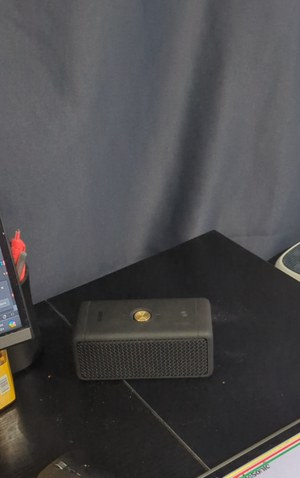
\includegraphics[width=0.31\linewidth]{ex_align_raw.jpg}\hfill
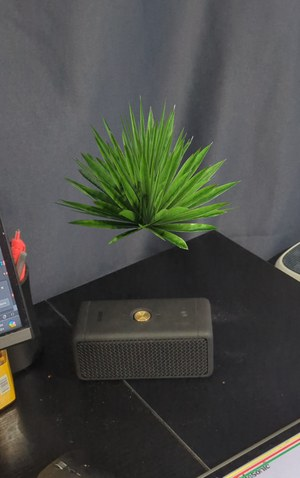
\includegraphics[width=0.31\linewidth]{ex_align_ar.jpg}\hfill
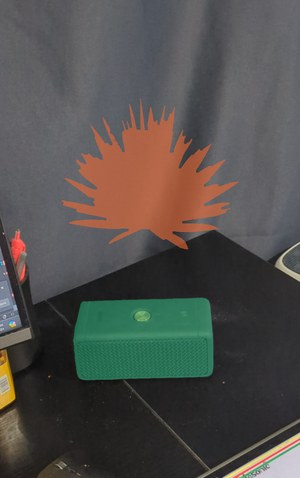
\includegraphics[width=0.31\linewidth]{ex_align_masks.jpg}
\caption{Par benigno do dataset de manipulação ($A=0$, $S=1$, $I=1$, logo $M=0$). Esquerda: $\Ir$.
Centro: $\Ia$, com uma planta virtual acima da caixa de som. Direita: a medida geométrica de
alinhamento (Seção~\ref{sec:hipoteses}): objeto detectado a partir do nome dado pelo Qwen3-VL-4B, em
verde, e conteúdo extraído pela diferença entre as imagens, em laranja. A separação de 142 pixels indica
$A=0$, mas o VLM havia respondido que o conteúdo estava alinhado.}
\label{fig:exemplo}
\end{figure}

% =====================================================================================================
\section{Metodologia}
\label{sec:metodo}

\subsection{Reimplementação e validação}
\label{sec:reconstrucao}
O repositório de Xiu \emph{et al.} traz o dataset e dois notebooks de demonstração com GPT-4o, mas não o
código que produz os resultados publicados. Faltam as linhas de base, as métricas e a geração das
máscaras $m_c$, e os notebooks divergem da descrição publicada em pontos que afetam o resultado (o de obstrução, por
exemplo, sorteia $\alpha$ entre 0,175 e 0,225 a cada imagem). Reimplementamos o pipeline a partir da
descrição publicada, com os prompts transcritos literalmente. Usamos o Grounding DINO aberto no lugar da
versão~1.5, disponível só por API.

Onde a descrição é omissa, tomamos decisões explícitas. A máscara $m_c$ é obtida comparando as duas
fotografias pixel a pixel: como $\Ir$ e $\Ia$ são capturadas do mesmo ponto de vista, os pixels em que
algum canal de cor difere mais de 30 níveis (numa escala de 0 a 255) pertencem ao conteúdo virtual e
recebem 1, e os demais recebem 0. Uma abertura morfológica remove pixels isolados de ruído, e um
fechamento preenche pequenos buracos. O dataset publica só 32 máscaras de conteúdo, sem indicar a que
pares pertencem; as nossas coincidem com elas (IoU mediano de 0,99). Na manipulação, as respostas do VLM
a cada fator, $\hat A$, $\hat S$ e $\hat I$, são lidas da primeira ocorrência de ``yes'' ou ``no'' nas
respostas 3, 4 e 5. O código guarda a resposta bruta do VLM, de modo que regras de decisão e métricas são
recalculadas sem consultar os modelos de novo.

Para validar a reimplementação, comparamos os métodos que não dependem do VLM e o mesmo VLM usado por Xiu \emph{et al.}
com os números publicados. O \emph{prior knowledge} acerta 93,8\% dos pares de obstrução, contra 93,1\%
publicados, e saliência e Canny ficam perto do acaso, como no original; isso confirma detector,
segmentador, $m_c$ e Eq.~\eqref{eq:obs}. Com o LLaVA-Next-8B, o ViDDAR tem 88,2\% contra 89,2\%, e o
só VLM, 51,3\% contra 55,2\%. Na manipulação, o LLaVA tem 38,6\% de acurácia, 37,0\% de precisão e
84,1\% de recall, contra 43,0\%, 39,8\% e 95,4\% publicados: o padrão é o mesmo (recall alto e precisão
baixa), e as diferenças são compatíveis com a quantização e a decodificação locais. Essa é a única
comparação direta com os números publicados.

\subsection{Modelos e execução}
Avaliamos cinco VLMs abertos de três famílias: Qwen3-VL-2B, Qwen3-VL-4B e Qwen3-VL-8B
(Instruct)~\cite{qwen3vl}, que mostram o efeito do tamanho dentro de uma família; LLaVA-Next-8B~\cite{llava},
o modelo aberto usado por Xiu \emph{et al.}; e Gemma~4 12B~\cite{gemma4}. Todos rodam localmente numa
GPU NVIDIA RTX 3060 de 12~GB: os dois menores em bf16 e os três maiores quantizados em 4 bits
(NF4~\cite{qlora}). A decodificação é determinística (greedy), as imagens são reduzidas a no máximo 1
megapixel e passadas na ordem $\Ir$, $\Ia$, e a resposta é limitada a 256 tokens na obstrução e a 768 na manipulação. Na obstrução, o VLM
leva de 1 a 3~s por par, e a geometria, 0,8~s; na manipulação, o questionário leva de 13 a 23~s por par.

\subsection{Dados}
Usamos os dois datasets publicados por Xiu \emph{et al.}, capturados em ambientes reais com um
aplicativo de RA para Android (Unity e ARCore) num smartphone. Na obstrução, formas geométricas virtuais
foram posicionadas aleatoriamente na cena; cada par tem um objeto-chave, cuja classe, máscara e situação
de obstrução foram rotuladas à mão. São 306 pares de 23 classes de objeto-chave (placas, extintores,
tomadas, facas, entre outras), dos quais 145 são ataques. Na manipulação, que exige alinhamento preciso
entre o conteúdo e o objeto, o conteúdo foi ancorado a uma imagem de calibração exibida num tablet e
rastreada pelo ARCore. São 114 pares de 10 combinações de conteúdo virtual e cena, com rótulos manuais de
$A$, $S$, $I$ e $M$ que satisfazem a Eq.~\eqref{eq:man} (Tabela~\ref{tab:composicao}). Os autores
validaram os rótulos com um estudo com 20 participantes. Quase todo par benigno tem
dois fatores verdadeiros (Tabela~\ref{tab:composicao}): para acertá-lo, o modelo precisa responder
``não'' exatamente ao fator que falha; um modelo que responde
``sim'' a tudo acusa ataque em todos eles. Há também poucos pares que testam a rejeição de $I$: só 11.

\begin{table}[!t]
\renewcommand{\arraystretch}{1.05}
\caption{Composição do dataset de manipulação pelos rótulos dos fatores}
\label{tab:composicao}
\centering
\footnotesize
\begin{tabular}{cccL{3.5cm}c}
\toprule
$A$ & $S$ & $I$ & Par & Pares \\
\midrule
1 & 1 & 1 & ataque ($M=1$) & 44 \\
0 & 1 & 1 & benigno: desalinhado & 32 \\
1 & 0 & 1 & benigno: textura artificial & 25 \\
1 & 1 & 0 & benigno: não sugere nada falso & 11 \\
0 & 0 & 1 & benigno: desalinhado e artificial & 2 \\
\bottomrule
\end{tabular}
\end{table}

\subsection{Convenções, métricas e testes}
\label{sec:metricas}
Nas duas tarefas, a classe positiva é o \textbf{ataque}, e o detector \textbf{dispara} quando acusa um.
Um falso positivo (FP) é disparar num par \textbf{benigno}, e um falso negativo (FN), não disparar num
ataque. Na manipulação, ``sim'' a um fator é uma condição a favor do ataque, então um viés de ``sim''
produz FP, e um de ``não'', FN. Além de acurácia, precisão e recall, as métricas de Xiu \emph{et al.},
reportamos a taxa de falsos positivos (FPR, fração dos benignos em que o detector dispara) e a de falsos
negativos (FNR, $1-$recall), com intervalos de Wilson~\cite{wilson}. Para comparar duas execuções nos
mesmos pares, como dois modelos ou uma execução e o detector trivial, usamos o teste exato de
McNemar~\cite{mcnemar1947,dietterich1998}, com $p<0{,}05$.

Na obstrução, o objeto-chave conta como \textbf{reconhecido} quando a máscara recortada a partir do nome
dado pelo VLM tem IoU $\geq 0{,}5$ com a verdadeira. Na manipulação, o índice de
Youden~\cite{youden1950} mede se a resposta do VLM sobre cada fator $F\in\{A,S,I\}$ depende do rótulo:
\begin{equation}
J_F = P(\hat F=\text{sim}\mid F=1) - P(\hat F=\text{sim}\mid F=0).
\label{eq:youden}
\end{equation}
$J_F=1$ é um juiz perfeito; $J_F=0$, um modelo cuja resposta não depende do fator, como um que diz
``sim'' sempre; e $J_F<0$, um que diz ``sim'' mais quando o fator é falso. Ao contrário da acurácia por
fator, $J_F$ não premia o viés para o rótulo majoritário.

\subsection{Atribuição de erros}
\label{sec:atrib}
\textbf{Obstrução.} Cada erro do pipeline é atribuído à primeira etapa que falhou: \emph{nada
detectado}, quando o Grounding DINO não encontra o nome; \emph{objeto errado}, quando a máscara
recortada tem IoU $<0{,}5$ com a verdadeira, isto é, o VLM nomeou outro objeto ou o detector achou outro;
e \emph{limiar}, quando o objeto certo foi recortado, mas a fração coberta ficou do lado errado de
$\alpha$. Se o \emph{prior knowledge} acerta a mesma amostra, o erro veio do nome dado pelo VLM; se também
erra, está na detecção, na segmentação, no limiar ou no rótulo.

\textbf{Manipulação.} Como o dataset rotula os três fatores, cada erro recebe uma causa, nesta ordem:
\emph{ilegível}, quando a decisão ou alguma resposta 3--5 não pôde ser interpretada (conta como erro e
nunca é descartada); \emph{conclusão}, quando a resposta 6 contradiz o que as respostas 3--5 implicam
(por exemplo, ``não'' a $I$ seguido de ``sim'' na conclusão); e \emph{percepção}, quando a conclusão segue
as respostas e o erro está nos fatores. Num falso positivo por percepção, o modelo disse ``sim'' aos
fatores cujo rótulo é 0; num falso negativo, disse ``não'' a algum fator verdadeiro. Cada causa é contada
sobre os pares em que pode ocorrer: aceitar um $A$ falso, por exemplo, só pode acontecer nos 34 pares
benignos com $A=0$, e rejeitar um fator verdadeiro, nos 44 ataques.

\subsection{Hipóteses e intervenções na manipulação}
\label{sec:hipoteses}
A literatura da Seção~\ref{sec:rel} sugere três origens para os erros da manipulação, e cada uma deu
origem a uma intervenção (Fig.~\ref{fig:prompts}). As variantes foram escritas a partir do prompt e das
definições de Xiu \emph{et al.}, e não dos pares em que os modelos erraram, e foram congeladas antes das
execuções completas. O prompt original é a variante \vpaper\ (P).
\begin{itemize}
\item \textbf{O prompt induz o ``sim''} (variante \vneutral, N). O prompt afirma que $\Ia$ foi criada
  ``adicionando conteúdo virtual'' e pede ao modelo que ``pense criativamente'' antes de negar $I$, como
  nas premissas embutidas que levam LLMs a concordar~\cite{sharma2024,pope}. A variante diz que $\Ia$
  ``pode conter'' conteúdo virtual e retira a instrução.
\item \textbf{A conclusão ignora as próprias respostas} (variante \vpd, PD). Como o raciocínio pode não
  determinar a resposta final~\cite{turpin2023}, a pergunta 6 pode contradizer as respostas 3--5, e
  responder tudo numa chamada pode fazer um ``sim'' puxar os outros. A variante faz uma chamada para o
  conteúdo e o objeto e uma chamada por fator, e a decisão $\hat A\wedge\hat S\wedge\hat I$ é calculada
  em código~\cite{khot2023}. Para separar os dois efeitos, aplicamos a mesma regra às respostas 3--5 do
  questionário original.
\item \textbf{O VLM julga mal o alinhamento} (medida geométrica). O fator $A$ é o mais geométrico dos
  três, e testamos se uma medida em pixels o julga melhor. Reaproveitamos os componentes da obstrução: o
  nome do objeto dado pelo VLM vai para o Grounding DINO e o SAM, que produzem $m_k$, e $m_c$ vem da
  diferença entre as imagens (Fig.~\ref{fig:exemplo}). A medida é a menor distância entre as duas
  máscaras, dividida pelo maior lado da caixa do conteúdo, e $\Ageo=1$ quando ela fica abaixo de um
  limiar escolhido por validação cruzada estratificada em 5 partições. A \textbf{decisão híbrida} combina
  o alinhamento medido pela geometria com os julgamentos do VLM sobre estilo e informação:
  $\Ageo\wedge\hat S\wedge\hat I$.
\end{itemize}

\begin{figure*}[!t]
\centering
\fbox{\begin{minipage}[t]{0.56\textwidth}\scriptsize
\textsf{\textbf{Prompt original (P), uma chamada com $\Ir$ e $\Ia$}}\\[2pt]\ttfamily\raggedright
Here are two images. The first one is a raw image, and the second one is an augmented image,
\textbf{created by adding some virtual content to the space.}\\
Please answer the following questions:\\
1. What is the virtual content in the augmented image?\\
2. What 'key object' is interacting with the virtual content? Avoid general terms like 'table surface'
or 'environment.'\\
3. Is the virtual content accurately aligned to the object, without a significant gap? Answer yes or
no, then explain why.\\
4. Does the virtual content have a relatively high-quality yet reasonable texture that blends it into
the real world? Answer yes or no, then explain why.\\
5. Do you think the interaction will make users believe the 'key object' has some false functionality
or information it does not have, or lose some true functionality or information it actually has?
\textbf{Think creatively, only say no if the combination has no specific semantic relation.} Answer yes
or no, then explain why.\\
6. If you answered 'yes' in all questions 3, 4, and 5, you must say 'yes.' Otherwise, you say 'no.'
\end{minipage}}\hfill
\fbox{\begin{minipage}[t]{0.40\textwidth}\scriptsize
\textsf{\textbf{Variante neutra (N)}: os dois trechos em negrito mudam}\\[2pt]\ttfamily\raggedright
... augmented image, which may contain virtual content added to the space.\\
(5. sem a frase ``Think creatively...'')\\[4pt]
\textsf{\textbf{Variante decomposta (PD): quatro chamadas}}\\[2pt]
Chamada 1: o preâmbulo de P e ``1. What is the virtual content...? 2. What 'key object'...?'', cada
resposta com até 4 palavras.\\[2pt]
Chamadas 2--4, uma por fator, com o preâmbulo de P e:\\
The virtual content is: \{content\}. The key object interacting with it is: \{key\_obj\}.\\
<pergunta 3, 4 ou 5 de P> Start your answer with yes or no, then explain why.\\[2pt]
Decisão: $\hat A\wedge\hat S\wedge\hat I$, calculada em código.
\end{minipage}}
\caption{Prompts da manipulação. À esquerda, o questionário de Xiu \emph{et al.}, transcrito
literalmente; à direita, o que muda em cada variante. As variantes foram derivadas do texto e das
definições originais, e não dos erros observados.}
\label{fig:prompts}
\end{figure*}

% =====================================================================================================
\section{Resultados: obstrução}
\label{sec:res-obs}

\begin{table}[!t]
\renewcommand{\arraystretch}{1.05}
\caption{Detecção de obstrução nos 306 pares (145 ataques), em \%, com $\alpha=0{,}25$, com os métodos
agrupados pelo papel do VLM. Em negrito, o melhor valor de cada linha}
\label{tab:obs}
\centering
\footnotesize
\setlength{\tabcolsep}{3.2pt}
\begin{tabular}{lccccc}
\toprule
 & Qwen 2B & Qwen 4B & Qwen 8B & LLaVA & Gemma \\
\midrule
\multicolumn{6}{l}{\textit{ViDDAR: o VLM nomeia o objeto, a geometria decide}} \\
\quad acurácia & 84,6 & 91,5 & \textbf{91,8} & 88,2 & 90,5 \\
\quad \scriptsize IC 95\% & \scriptsize 80--88 & \scriptsize 88--94 & \scriptsize 88--94 & \scriptsize 84--91 & \scriptsize 87--93 \\
\quad precisão & 90,8 & 95,4 & \textbf{97,6} & 91,6 & 97,5 \\
\quad recall & 75,2 & \textbf{86,2} & 84,8 & 82,8 & 82,1 \\
\quad FPR & 6,8 & 3,7 & \textbf{1,9} & 6,8 & \textbf{1,9} \\
\quad objeto reconhecido & 72,5 & \textbf{89,9} & 85,0 & 76,1 & 88,6 \\
\midrule
\multicolumn{6}{l}{\textit{Só VLM (end-to-end): o VLM nomeia o objeto e decide}} \\
\quad acurácia & 45,1 & 72,9 & 73,5 & 51,3 & \textbf{81,7} \\
\quad recall & 81,4 & 66,9 & \textbf{84,8} & 8,3 & 80,7 \\
\quad FPR & 87,6 & 21,7 & 36,6 & \textbf{9,9} & 17,4 \\
\midrule
\multicolumn{6}{l}{\textit{ViDDAR com outro prompt de objeto-chave (acurácia)}} \\
\quad underdetailed & 82,7 & \textbf{85,6} & 82,7 & 82,7 & 80,1 \\
\quad greedy & 88,9 & 90,5 & \textbf{92,2} & 87,3 & 90,5 \\
\midrule
\multicolumn{6}{l}{\textit{Sem VLM (acurácia)}} \\
\quad prior knowledge & \multicolumn{5}{c}{93,8 (nome verdadeiro do objeto)} \\
\quad saliência / Canny & \multicolumn{5}{c}{52,3 / 49,7} \\
\bottomrule
\multicolumn{6}{L{8.2cm}}{\scriptsize Qwen: Qwen3-VL; LLaVA: LLaVA-Next-8B; Gemma: Gemma~4 12B.
Objeto reconhecido: a máscara recortada a partir do nome dado pelo VLM tem IoU $\geq 0{,}5$ com a
verdadeira. Underdetailed: prompt mínimo; greedy: o VLM pode listar vários objetos.}
\end{tabular}
\end{table}

\subsection{Os VLMs abertos sustentam o detector de obstrução}
A Tabela~\ref{tab:obs} responde à QP1 para a obstrução: os cinco modelos sustentam o detector, e três
deles, o Qwen3-VL-4B, o Qwen3-VL-8B e o Gemma~4, ficam perto do limite superior do pipeline e empatam
entre si no teste de McNemar. O 4B e o 8B não se distinguem nem do \emph{prior knowledge}, que recebe o
nome verdadeiro do objeto: com esses modelos, escolher o objeto-chave deixa de ser o gargalo. O
Qwen3-VL-2B fica
significativamente atrás dos demais, e a linha ``objeto reconhecido'' mostra por quê: é o modelo que
mais nomeia um objeto diferente do anotado. Na família Qwen, o tamanho ajuda do 2B para o 4B, mas não do
4B para o 8B, que quase não discordam entre si. No outro extremo, saliência e Canny ficam perto do acaso:
sem saber qual objeto importa na cena, heurísticas visuais não detectam obstrução, e é essa escolha que o
VLM fornece.

Em todos os modelos, o detector é conservador: a precisão é alta e a FPR é baixa, mas o recall é menor,
ou seja, ele raramente acusa uma obstrução inexistente e, quando erra, em geral deixa passar uma real.

\subsection{Separar reconhecimento e decisão}
Nos cinco modelos, o ViDDAR supera com significância o só VLM. Sem a regra geométrica, cada modelo revela uma tendência própria, que a geometria antes neutralizava: o
Qwen3-VL-2B acusa obstrução em quase todas as amostras, e o LLaVA-Next-8B em quase nenhuma; o Qwen3-VL-8B
tende ao ``sim'', e o Qwen3-VL-4B, ao ``não''. O Gemma~4 é a exceção: acusa obstrução em tantas amostras
quantas estão de fato obstruídas e tem o melhor resultado só VLM. Como ele não é o modelo que melhor
reconhece o objeto, sua vantagem está em decidir.

\subsection{O prompt define o que é um objeto-chave}
O \emph{underdetailed} piora significativamente quatro dos cinco modelos. Sem o papel, a menção a
segurança e os exemplos, os modelos nomeiam objetos salientes,
mas irrelevantes: ``door'' passa a ser a resposta mais frequente do Gemma~4 e do Qwen3-VL-2B, e o Gemma~4
passa a reconhecer o objeto-chave com muito menos frequência. O papel e os exemplos não ensinam o modelo a
ver melhor; eles dizem \emph{que tipo} de objeto conta como importante. O \emph{greedy} empata com o
ViDDAR em quase todos os modelos. A exceção é o Qwen3-VL-2B, que melhora com significância: para o modelo
que mais erra o objeto, listar vários candidatos compensa a escolha errada de um só.

\subsection{De onde vêm os erros}
\label{sec:res-obs-erros}

\begin{table}[!t]
\renewcommand{\arraystretch}{1.05}
\caption{Obstrução: erros do pipeline por etapa (Seção~\ref{sec:atrib}). Entre parênteses, quantas
dessas amostras o \emph{prior knowledge}, que recebe o nome verdadeiro, também erra}
\label{tab:obs-causas}
\centering
\footnotesize
\setlength{\tabcolsep}{3.2pt}
\begin{tabular}{llccccc}
\toprule
Erro & Etapa & Qwen 2B & 4B & 8B & LLaVA & Gemma \\
\midrule
FP & objeto errado & 11 (0) & 6 (0) & 3 (0) & 11 (0) & 3 (0) \\
\midrule
\multirow{3}{*}{FN} & nada detectado & 3 (0) & 0 & 0 & 0 & 0 \\
 & objeto errado & 17 (2) & 5 (3) & 7 (2) & 15 (6) & 12 (4) \\
 & limiar & 16 (14) & 15 (14) & 15 (14) & 10 (9) & 14 (13) \\
\bottomrule
\multicolumn{7}{l}{\scriptsize De 161 pares benignos (FP) e 145 ataques (FN). O \emph{prior} tem 1 FP e 18 FN.}
\end{tabular}
\end{table}

A Tabela~\ref{tab:obs-causas} responde à QP2 para a obstrução, e os dois tipos de erro contam histórias
distintas.

\textbf{Falsos positivos: qual objeto importa.} Todos os falsos positivos são de reconhecimento, e o
\emph{prior knowledge} acerta todas essas amostras. Em cada caso, o VLM nomeia um objeto diferente do
anotado, e o conteúdo virtual cobre esse outro objeto. Os casos se concentram em poucas cenas com mais de
um objeto plausível (Fig.~\ref{fig:obs-fp}): diante de uma placa de advertência pregada numa porta, quatro
modelos nomeiam a porta (``black door with sign''); diante de uma panela fervendo, quatro nomeiam o
queimador ou o fogão (``glowing red burner'', ``black stove''). Fora dessas cenas e das tomadas, os três
melhores modelos quase não têm falsos positivos. O Qwen3-VL-2B tem um modo de falha próprio: com
frequência ele responde ``red box'', copiando o exemplo do prompt, e cerca de metade dos seus falsos
positivos vem disso (Fig.~\ref{fig:redbox}). Esses falsos positivos, portanto, não vêm da percepção
visual nem da geometria, e sim de uma escolha que o prompt não especifica.

\begin{figure}[!t]
\centering
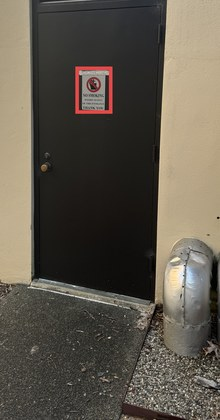
\includegraphics[height=2.75cm]{ex_fp_warning-sign_002_raw.jpg}\hspace{1pt}%
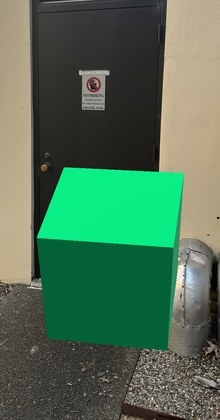
\includegraphics[height=2.75cm]{ex_fp_warning-sign_002_ar.jpg}\hfill
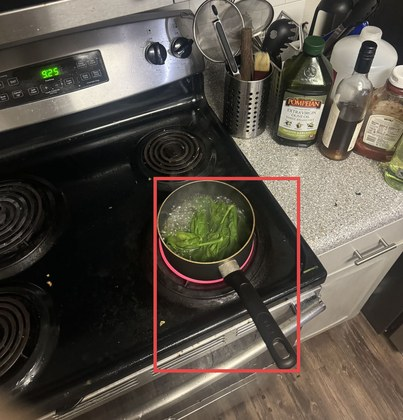
\includegraphics[height=2.75cm]{ex_fp_boiling-pot_010_raw.jpg}\hspace{1pt}%
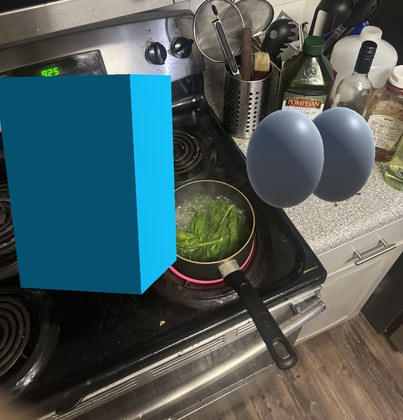
\includegraphics[height=2.75cm]{ex_fp_boiling-pot_010_ar.jpg}
\caption{Dois pares benignos de obstrução em que quatro dos cinco VLMs disparam. Em cada par, à
esquerda, $\Ir$ com o objeto-chave anotado (contorno vermelho) e, à direita, $\Ia$. Esquerda: a placa de
advertência; os modelos nomeiam a porta, coberta em 41\% pelo cubo virtual. Direita: a panela; os modelos
nomeiam o queimador ou o fogão, cobertos em 25\% a 47\%.}
\label{fig:obs-fp}
\end{figure}

\begin{figure}[!t]
\centering
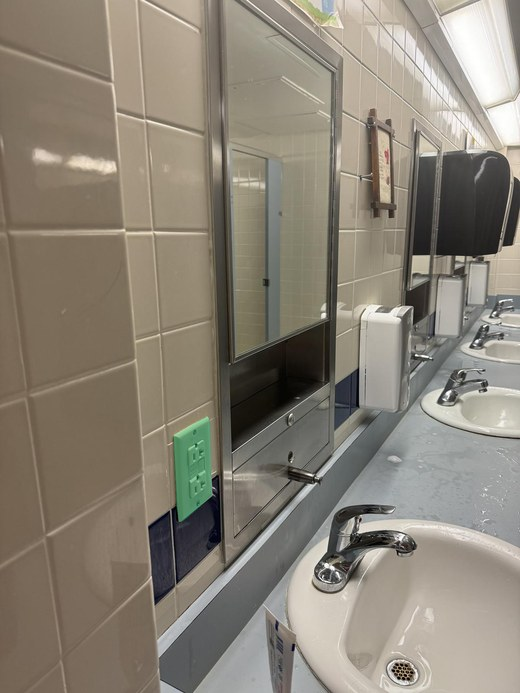
\includegraphics[height=3.6cm]{ex_obs_key.jpg}\hspace{4pt}%
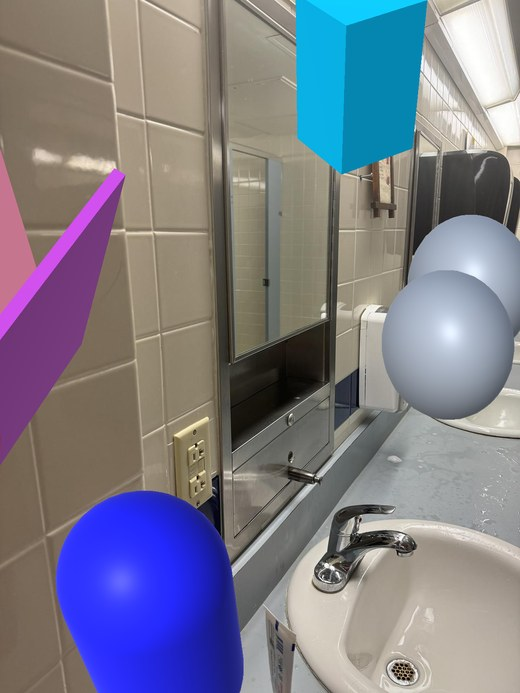
\includegraphics[height=3.6cm]{ex_obs_ar.jpg}
\caption{Falso positivo do Qwen3-VL-2B por cópia do prompt. Esquerda: $\Ir$, com o objeto-chave anotado
(a tomada) em verde. Direita: $\Ia$. O VLM respondeu ``red box'', o exemplo do prompt. O Grounding DINO
procurou esse nome em $\Ir$ e devolveu outro objeto (IoU de 0,00 com a tomada), 45\% coberto pelo
conteúdo virtual. Pela Eq.~\eqref{eq:obs}, o pipeline acusou obstrução de um objeto que não era o
objeto-chave; a tomada não está coberta.}
\label{fig:redbox}
\end{figure}

\textbf{Falsos negativos: cobertura logo abaixo de $\alpha$.} Os falsos negativos são o erro dominante
e, ao contrário dos falsos positivos, em geral não dependem do VLM. A maior parte é de limiar: o objeto
certo foi recortado, mas a fração coberta ficou logo abaixo de $\alpha$. O \emph{prior knowledge} erra
quase todas essas amostras, e várias se repetem nos cinco modelos. Coerentemente, a acurácia de todos os
modelos, e também a do \emph{prior}, seria maior com $\alpha=0{,}20$. O mesmo acontece sem nenhum modelo:
aplicando a Eq.~\eqref{eq:obs} às máscaras verdadeiras dos objetos, os rótulos concordam mais com a regra
em $\alpha=0{,}20$ do que em $0{,}25$, o valor que Xiu \emph{et al.} identificaram como fronteira
aproximada entre pares obstruídos e não obstruídos. A explicação provável é que as nossas máscaras $m_c$
sejam um pouco menores que as usadas na rotulagem. Mantivemos $\alpha=0{,}25$, porque escolher o limiar
no conjunto de teste seria otimista, e a ordem dos modelos não muda com $\alpha$.

% =====================================================================================================
\section{Resultados: manipulação de informação}
\label{sec:res-man}

\begin{table*}[!t]
\renewcommand{\arraystretch}{1.0}
\caption{Detecção de manipulação nos 114 pares (44 ataques), em \%, com o prompt original (P) e as
variantes neutra (N) e decomposta (PD) da Fig.~\ref{fig:prompts}. ``vs.~trivial'': comparação, pelo McNemar, com o detector que nunca
dispara (61,4\%); n.s. = sem diferença significativa. $J$: índice de Youden de cada fator
(Eq.~\ref{eq:youden}), 0 quando a resposta não depende do fator}
\label{tab:man}
\centering
\footnotesize
\setlength{\tabcolsep}{4.2pt}
\begin{tabular}{llccccccccc}
\toprule
Modelo & Variante & Acurácia & Precisão & Recall & FPR & FNR & vs.~trivial & $J_A$ & $J_S$ & $J_I$ \\
\midrule
\multirow{3}{*}{Qwen3-VL-2B}
 & P  & 38,6 & 38,2 & 95,5 & 97,1 & 4,5 & abaixo & $-$0,03 & $-$0,02 & 0,00 \\
 & N  & 48,2 & 42,7 & 93,2 & 78,6 & 6,8 & n.s. & $-$0,03 & $-$0,01 & 0,00 \\
 & PD & 37,7 & 37,4 & 90,9 & 95,7 & 9,1 & abaixo & $-$0,03 & 0,07 & 0,00 \\
\midrule
\multirow{3}{*}{Qwen3-VL-4B}
 & P  & 61,4 & 50,0 & 6,8 & 4,3 & 93,2 & n.s. & 0,09 & 0,31 & $-$0,30 \\
 & N  & 61,4 & -- & 0,0 & 0,0 & 100 & n.s. & 0,28 & 0,41 & $-$0,20 \\
 & PD & 73,7 & 93,8 & 34,1 & 1,4 & 65,9 & \textbf{acima} & 0,25 & 0,22 & $-$0,01 \\
\midrule
\multirow{3}{*}{Qwen3-VL-8B}
 & P  & 37,7 & 38,1 & 97,7 & 100 & 2,3 & abaixo & 0,48 & 0,25 & $-$0,01 \\
 & N  & 60,5 & 49,4 & 90,9 & 58,6 & 9,1 & n.s. & 0,48 & 0,22 & 0,08 \\
 & PD & 69,3 & 61,5 & 54,5 & 21,4 & 45,5 & n.s. & 0,32 & 0,50 & $-$0,09 \\
\midrule
\multirow{3}{*}{LLaVA-Next-8B}
 & P  & 38,6 & 37,0 & 84,1 & 90,0 & 15,9 & abaixo & $-$0,13 & $-$0,02 & 0,00 \\
 & N  & 53,5 & 42,6 & 59,1 & 50,0 & 40,9 & n.s. & 0,05 & $-$0,03 & 0,00 \\
 & PD & 63,2 & 55,0 & 25,0 & 12,9 & 75,0 & n.s. & 0,05 & $-$0,06 & 0,00 \\
\midrule
\multirow{3}{*}{Gemma 4 12B}
 & P  & 55,3 & 46,2 & 95,5 & 70,0 & 4,5 & n.s. & 0,20 & 0,16 & 0,25 \\
 & N  & 59,6 & 48,2 & 61,4 & 41,4 & 38,6 & n.s. & 0,24 & 0,31 & 0,18 \\
 & PD & 61,4 & -- & 0,0 & 0,0 & 100 & n.s. & 0,35 & 0,00 & 0,21 \\
\bottomrule
\multicolumn{11}{l}{\scriptsize Precisão indefinida (--) quando o modelo nunca dispara. O $J_I$ usa só os 11 pares com $I=0$ e é pouco preciso.}
\end{tabular}
\end{table*}

\subsection{Nenhum modelo supera o detector trivial}
A Tabela~\ref{tab:man} responde à QP1 para a manipulação, e a resposta é negativa. Com o prompt original,
nenhum modelo acerta significativamente mais que o detector que nunca dispara, e três ficam
significativamente \emph{abaixo} dele: o Qwen3-VL-2B, o Qwen3-VL-8B e o LLaVA-Next-8B disparam em quase
todos os pares benignos. O Qwen3-VL-4B empata com o detector trivial pelo motivo oposto, porque quase
nunca dispara, e o Gemma~4 fica entre os dois extremos.

A acurácia esconde o que acontece. Em quatro dos cinco modelos, o recall e a FPR ficam próximos: o modelo
dispara nos ataques e nos pares benignos na mesma proporção, como um detector que não olha as imagens.
Só o Gemma~4 dispara mais nos ataques que nos benignos, um sinal fraco de discriminação. Como há mais
pares benignos que ataques, qualquer deslocamento para o ``não'' aumenta a acurácia sem que o modelo
discrimine melhor; por isso, nas variantes, a comparação com o detector trivial é mais informativa que o
ganho de acurácia. O LLaVA-Next-8B decomposto, por exemplo, ganha acurácia porque passa a perder a maior
parte dos ataques. Das 15 configurações, só uma supera o detector trivial: o Qwen3-VL-4B decomposto, que
detecta uma parte dos ataques quase sem alarmes falsos. O Qwen3-VL-8B decomposto é o detector mais
equilibrado entre recall e FPR, mas não se distingue do trivial.

\subsection{As causas dos erros}
\label{sec:res-man-causas}

\begin{table}[!t]
\renewcommand{\arraystretch}{1.05}
\caption{Manipulação: causas dos erros com o prompt original (Seção~\ref{sec:atrib}). Cada célula é o
número de erros sobre o número de pares em que a causa pode ocorrer}
\label{tab:causas}
\centering
\footnotesize
\setlength{\tabcolsep}{2.6pt}
\begin{tabular}{llccccc}
\toprule
 & Causa & Qwen 2B & 4B & 8B & LLaVA & Gemma \\
\midrule
\multirow{4}{*}{FP} & conclusão & 68/70 & 0/70 & 44/70 & 0/70 & 0/70 \\
 & aceitou $A$ falso & 0/34 & 2/34 & 10/34 & 33/34 & 24/34 \\
 & aceitou $S$ falso & 0/27 & 1/27 & 11/27 & 24/27 & 20/27 \\
 & aceitou $I$ falso & 0/11 & 0/11 & 5/11 & 8/11 & 7/11 \\
\midrule
\multirow{5}{*}{FN} & ilegível & 2/44 & 0/44 & 0/44 & 0/44 & 0/44 \\
 & conclusão & 0/44 & 0/44 & 0/44 & 0/44 & 1/44 \\
 & rejeitou $A$ verdadeiro & 0/44 & 3/44 & 1/44 & 7/44 & 1/44 \\
 & rejeitou $S$ verdadeiro & 0/44 & 3/44 & 1/44 & 7/44 & 0/44 \\
 & rejeitou $I$ verdadeiro & 0/44 & 38/44 & 1/44 & 0/44 & 0/44 \\
\midrule
\multicolumn{2}{l}{Total FP / FN} & 68 / 2 & 3 / 41 & 70 / 1 & 63 / 7 & 49 / 2 \\
\bottomrule
\multicolumn{7}{L{8.2cm}}{\scriptsize Um erro em que o modelo julga mal dois fatores conta nas duas
linhas, por isso as linhas podem somar mais que o total. Nenhum falso positivo foi ilegível.}
\end{tabular}
\end{table}

A Tabela~\ref{tab:causas} responde à QP2 para a manipulação: não há uma causa comum, e cada modelo tem a
sua.

\textbf{Conclusão que contradiz as respostas (Qwen3-VL-2B e Qwen3-VL-8B).} Quase todos os falsos
positivos do Qwen3-VL-2B são de conclusão: ele responde ``não'' a $I$ em todos os pares, o que deveria
levar a ``não'' na pergunta 6, e mesmo assim conclui ``sim'' na grande maioria deles, muitas vezes
afirmando ter dito ``sim'' às perguntas 3 a 5. O Qwen3-VL-8B faz o mesmo de forma mais clara: responde
``Yes.'' na pergunta 6 em praticamente todos os pares, inclusive depois de negar o alinhamento, como num
par benigno com $A=0$: ``\emph{3. No. The virtual plant is positioned floating in the air directly above
the hard drive, with a clear gap [\dots] 6. Yes.}''

\textbf{Aceitação de alinhamento e estilo ruins (LLaVA-Next-8B e Gemma~4).} Nesses dois modelos, a
conclusão segue as respostas, mas as respostas aceitam quase tudo: os dois aceitam o alinhamento e o
estilo na maior parte dos pares em que esses fatores são falsos. O LLaVA chega a descrever o
desalinhamento e, logo depois, negá-lo: ``\emph{1. [\dots] a cup of coffee with a saucer, floating above
the fan. [\dots] 3. Yes, the virtual content is accurately aligned to the fan without a significant
gap.}''

\textbf{Leitura restritiva de $I$ (Qwen3-VL-4B).} O Qwen3-VL-4B quase não dispara em pares benignos,
mas rejeita $I$ na maior parte dos ataques. Ele identifica o conteúdo e o objeto, mas entende ``informação
falsa'' como algo absurdo e trata adições plausíveis como inofensivas: uma cesta virtual num patinete
seria ``um acessório plausível''. Para o método de referência é o contrário: é a plausibilidade que faz o
usuário acreditar que a cesta existe. A FPR baixa desse modelo, portanto, não é mérito: ele percebe mal o
alinhamento ($J_A$ próximo de zero), e é a rejeição de $I$ que barra os pares benignos.

\textbf{Os modelos percebem os fatores?} As colunas $J$ da Tabela~\ref{tab:man} respondem. No Qwen3-VL-2B e no LLaVA-Next-8B, $J$ fica
próximo de zero em todos os fatores e variantes: esses modelos respondem de forma quase igual a pares
alinhados e desalinhados, realistas e artificiais, e as variantes só mudam a frequência com que dizem
``sim''. Na família Qwen, o tamanho melhora a percepção do alinhamento, e o Qwen3-VL-8B é o modelo que
melhor a distingue. Nenhum modelo, porém, distingue $I$: $J_I$ fica próximo de zero ou negativo em quase
todas as configurações, e só o Gemma~4 tem valores positivos em todas, com intervalos largos. Como $I$ é
verdadeiro na grande maioria dos pares, aceitar $I$ sempre é a estratégia que mais acerta, e é o que
quatro dos cinco modelos fazem na variante decomposta; na prática, o detector se reduz a $\hat A\wedge\hat S$.

\subsection{O que as intervenções corrigem}
\label{sec:res-hip}
\textbf{O prompt induz o ``sim'': confirmada nos modelos que disparam demais.} Com a variante neutra, a
FPR cai e a acurácia sobe em todos os modelos que disparavam demais: o prompt original empurra os modelos
para o ``sim''. No Qwen3-VL-8B, que percebe os fatores, a queda de falsos positivos quase não custa
ataques; no LLaVA-Next-8B e no Gemma~4, ela vem acompanhada de um aumento parecido de falsos negativos.

\textbf{A conclusão ignora as respostas: confirmada, e é o principal problema do Qwen3-VL-8B.} A variante
decomposta elimina por construção o erro de conclusão e dá os maiores ganhos de acurácia sobre o prompt
original, no Qwen3-VL-4B, no Qwen3-VL-8B e no LLaVA-Next-8B, este à custa do recall. No lugar da
conclusão, porém, aparece o viés de cada pergunta isolada. O Qwen3-VL-4B e o Gemma~4 passam a rejeitar o
estilo; o Gemma descreve o conteúdo como ``a 2D sticker placed over the image'' em todos os pares e vira
um detector que nunca dispara. O LLaVA passa a rejeitar o alinhamento na maior parte dos ataques. Para
isolar o efeito de quem decide (Seção~\ref{sec:hipoteses}), aplicamos a regra
$\hat A\wedge\hat S\wedge\hat I$ às respostas do questionário original. No Qwen3-VL-8B, cuja resposta 6
contradiz a regra em muitos pares, essa troca corrige quase todos os falsos positivos de conclusão e
dobra a acurácia, embora ainda sem superar significativamente o detector trivial. O Qwen3-VL-8B
percebe o alinhamento e o estilo razoavelmente bem, mas ignora as próprias respostas na hora de decidir.
No Qwen3-VL-2B, a mesma troca leva ao próprio detector trivial, porque ele nega $I$ sempre. Nos outros
três modelos, a resposta 6 já concorda com a regra em quase todos os pares.

\textbf{O VLM julga mal o alinhamento: confirmada no fator, não na decisão.} A medida geométrica julga
$A$ melhor que o VLM em quatro dos cinco modelos, e o Gemma~4 empata (Tabela~\ref{tab:c2});
independentemente do limiar, a distância separa razoavelmente os pares alinhados dos desalinhados. Na
decisão, porém, a decisão híbrida só melhora com significância no LLaVA-Next-8B, e por troca: os falsos
positivos caem, mas os falsos negativos sobem quase na mesma proporção. Um $A$ melhor ajuda pouco porque, de novo, a decisão é uma
conjunção: onde $S$ ou $I$ já impedem o disparo, como no Qwen3-VL-2B e no Qwen3-VL-4B, $A$ não muda nada;
onde o VLM aceita tudo, a geometria corta falsos positivos, mas também ataques, porque a própria medida
ainda erra parte dos pares.

\begin{table}[!t]
\renewcommand{\arraystretch}{1.05}
\caption{Manipulação: alinhamento geométrico com o prompt original. Acerto no fator $A$ e acurácia da
decisão. A decisão híbrida $\Ageo\wedge\hat S\wedge\hat I$ é comparada com a regra
$\hat A\wedge\hat S\wedge\hat I$ sobre as respostas do próprio VLM, o que isola o efeito do $A$
geométrico}
\label{tab:c2}
\centering
\footnotesize
\setlength{\tabcolsep}{4pt}
\begin{tabular}{lcccc}
\toprule
 & \multicolumn{2}{c}{Acerto em $A$ (\%)} & \multicolumn{2}{c}{Acurácia da decisão (\%)} \\
\cmidrule(lr){2-3}\cmidrule(lr){4-5}
Modelo & VLM & geometria & $\hat A\wedge\hat S\wedge\hat I$ & híbrida \\
\midrule
Qwen3-VL-2B   & 70 & \textbf{79} & 61,4 & 61,4 \\
Qwen3-VL-4B   & 62 & \textbf{76} & 61,4 & 61,4 \\
Qwen3-VL-8B   & 75 & \textbf{80} & 75,4 & 78,1 \\
LLaVA-Next-8B & 60 & \textbf{65} & 38,6 & \textbf{52,6}$^{*}$ \\
Gemma 4 12B   & 74 & 73 & 54,4 & 59,6 \\
\bottomrule
\multicolumn{5}{L{7.4cm}}{\scriptsize $^{*}$Única diferença significativa entre as duas decisões
(McNemar, $p=0{,}036$; nas demais, $p\geq 0{,}36$).}
\end{tabular}
\end{table}

% =====================================================================================================
\section{Discussão}
\label{sec:disc}

\textbf{O que separa as duas tarefas é quem decide.} Os mesmos VLMs que vão bem na obstrução não
superam o detector trivial na manipulação, e a diferença está no papel do VLM: na obstrução, ele dá uma resposta curta e
localizada (um nome), e uma regra explícita decide; quando decide sozinho, no método só VLM, aparecem os
mesmos vieses de ``sim'' e de ``não'' observados na manipulação. Na manipulação, os melhores resultados
também vieram de tirar a decisão do VLM. Para quem projeta esses detectores com modelos pequenos, a
lição é usar o VLM como fonte de julgamentos simples e verificáveis, e não como juiz da decisão final.

\textbf{Os falsos positivos têm naturezas diferentes nas duas tarefas.} Na obstrução, eles são poucos,
interpretáveis e vêm, na maior parte, de ambiguidade semântica: em cenas com mais de um candidato razoável, o VLM escolhe
um diferente do anotado. Corrigi-los exige especificar melhor o que é o objeto-chave, no prompt ou no
rótulo, e não um modelo maior. Na manipulação, os falsos positivos são sistemáticos e vêm de vieses do
modelo, como a concordância com o prompt e a conclusão que ignora as próprias respostas, ou de percepção
fraca dos fatores. Intervenções no prompt e na forma de decidir só os reduzem sem custo nos modelos que
percebem os fatores, como o Qwen3-VL-8B ($J_A=0{,}48$); no LLaVA-Next-8B ($J_A\approx 0$), apenas trocam
falsos positivos por falsos negativos.

\textbf{Escala ajuda, mas não resolve o fator semântico.} Na família Qwen, o modelo maior reconhece
melhor o objeto-chave e percebe melhor o alinhamento e o estilo, mas, na manipulação, esse ganho só
aparece quando a conclusão sai do VLM. O fator $I$, que distingue um ataque
de um conteúdo apenas bem encaixado, não é medido de forma confiável por nenhum modelo, e o dataset também
o testa mal. Um benchmark para essa tarefa deveria equilibrar as
combinações de fatores e reportar FPR, FNR e a comparação com o detector trivial, e não só a acurácia.

% =====================================================================================================
\section{Limitações}
\label{sec:lim}

Os datasets são pequenos, e as conclusões sobre $I$ se apoiam em só 11 pares. As variantes de prompt e a
regra $\hat A\wedge\hat S\wedge\hat I$ foram avaliadas nos mesmos dados, sem conjunto de teste separado,
e, com vários testes, algum $p<0{,}05$ pode ser acaso. Os três maiores VLMs rodam em 4 bits, há uma única
execução por configuração, e a comparação com Xiu \emph{et al.} usa os números publicados, sem teste
pareado. As máscaras $m_c$ obtidas pela diferença de pixels só valem para pares alinhados pixel a pixel;
na obstrução, a categoria ``objeto errado'' mistura erros do VLM e do detector; e os fatores da
manipulação são lidos do texto livre por regras.

% =====================================================================================================
\section{Conclusão}

Avaliamos cinco VLMs abertos, executados localmente, nos dois detectores do ViDDAR. Na obstrução, o pipeline é robusto à troca do VLM, e os poucos falsos positivos vêm da escolha de outro
objeto plausível em cenas ambíguas. Na manipulação, nenhum modelo supera um detector que nunca dispara;
a causa dominante dos erros muda de modelo para modelo, as intervenções só ajudam os que percebem os
fatores, e nenhum distingue o fator semântico que define o ataque. Nas duas tarefas, o detector funciona melhor quando a decisão
final não fica com o VLM. Como próximos passos, propomos validar as configurações em dados novos, com
mais pares benignos em que $I$ é falso, e especificar no prompt como escolher entre objetos-chave
concorrentes.\label{fim-texto}

\begin{thebibliography}{99}

\bibitem{viddar}
Y.~Xiu, T.~Scargill, and M.~Gorlatova, ``{ViDDAR}: Vision language model-based task-detrimental
content detection for augmented reality,'' \emph{IEEE Trans. Vis. Comput. Graphics}, vol.~31, no.~5,
pp. 3194--3203, 2025, doi: 10.1109/TVCG.2025.3549147.

\bibitem{roesner2014}
F.~Roesner, T.~Kohno, and D.~Molnar, ``Security and privacy for augmented reality systems,''
\emph{Commun. ACM}, vol.~57, no.~4, pp. 88--96, 2014.

\bibitem{arya}
K.~Lebeck, K.~Ruth, T.~Kohno, and F.~Roesner, ``Securing augmented reality output,'' in \emph{Proc.
IEEE Symp. Security Privacy (SP)}, 2017, pp. 320--337.

\bibitem{cheng2023}
K.~Cheng, J.~F. Tian, T.~Kohno, and F.~Roesner, ``Exploring user reactions and mental models towards
perceptual manipulation attacks in mixed reality,'' in \emph{Proc. USENIX Security Symp.}, 2023.

\bibitem{vimsense}
Y.~Xiu and M.~Gorlatova, ``Detecting visual information manipulation attacks in augmented reality: A
multimodal semantic reasoning approach,'' \emph{IEEE Trans. Vis. Comput. Graphics}, 2025, preprint
arXiv:2507.20356.

\bibitem{duan2025}
L.~Duan, Y.~Xiu, and M.~Gorlatova, ``Advancing the understanding and evaluation of {AR}-generated
scenes: When vision-language models shine and stumble,'' in \emph{Proc. IEEE Conf. Virtual Reality 3D
User Interfaces Abstracts Workshops (VRW)}, 2025.

\bibitem{pope}
Y.~Li, Y.~Du, K.~Zhou, J.~Wang, W.~X. Zhao, and J.-R. Wen, ``Evaluating object hallucination in large
vision-language models,'' in \emph{Proc. Conf. Empirical Methods Natural Lang. Process. (EMNLP)},
2023.

\bibitem{sharma2024}
M.~Sharma \emph{et al.}, ``Towards understanding sycophancy in language models,'' in \emph{Proc. Int.
Conf. Learn. Represent. (ICLR)}, 2024.

\bibitem{turpin2023}
M.~Turpin, J.~Michael, E.~Perez, and S.~R. Bowman, ``Language models don't always say what they think:
Unfaithful explanations in chain-of-thought prompting,'' in \emph{Adv. Neural Inf. Process. Syst.
(NeurIPS)}, vol.~36, 2023.

\bibitem{zheng2023}
L.~Zheng \emph{et al.}, ``Judging {LLM}-as-a-judge with {MT-Bench} and {Chatbot Arena},'' in \emph{Adv.
Neural Inf. Process. Syst. (NeurIPS), Datasets and Benchmarks Track}, vol.~36, 2023.

\bibitem{khot2023}
T.~Khot, H.~Trivedi, M.~Finlayson, Y.~Fu, K.~Richardson, P.~Clark, and A.~Sabharwal, ``Decomposed
prompting: A modular approach for solving complex tasks,'' in \emph{Proc. Int. Conf. Learn. Represent.
(ICLR)}, 2023.

\bibitem{groundingdino}
S.~Liu \emph{et al.}, ``Grounding {DINO}: Marrying {DINO} with grounded pre-training for open-set
object detection,'' in \emph{Proc. Eur. Conf. Comput. Vis. (ECCV)}, 2024, preprint arXiv:2303.05499.

\bibitem{sam}
A.~Kirillov \emph{et al.}, ``Segment anything,'' in \emph{Proc. IEEE/CVF Int. Conf. Comput. Vis.
(ICCV)}, 2023, pp. 4015--4026.

\bibitem{hou2007}
X.~Hou and L.~Zhang, ``Saliency detection: A spectral residual approach,'' in \emph{Proc. IEEE Conf.
Comput. Vis. Pattern Recognit. (CVPR)}, 2007.

\bibitem{canny}
J.~Canny, ``A computational approach to edge detection,'' \emph{IEEE Trans. Pattern Anal. Mach.
Intell.}, vol.~PAMI-8, no.~6, pp. 679--698, 1986.

\bibitem{qwen3vl}
Qwen Team, ``{Qwen3-VL} model cards (2B, 4B and 8B Instruct),'' Hugging Face, 2025. [Online]. Available:
\url{https://huggingface.co/Qwen/Qwen3-VL-8B-Instruct}

\bibitem{llava}
H.~Liu, C.~Li, Q.~Wu, and Y.~J. Lee, ``Visual instruction tuning,'' in \emph{Adv. Neural Inf.
Process. Syst. (NeurIPS)}, vol.~36, 2023.

\bibitem{gemma4}
Google DeepMind, ``Gemma 4 model card (12B instruction-tuned),'' Hugging Face. [Online]. Available:
\url{https://huggingface.co/google/gemma-4-12B-it}

\bibitem{qlora}
T.~Dettmers, A.~Pagnoni, A.~Holtzman, and L.~Zettlemoyer, ``{QLoRA}: Efficient finetuning of
quantized {LLMs},'' in \emph{Adv. Neural Inf. Process. Syst. (NeurIPS)}, vol.~36, 2023.

\bibitem{wilson}
E.~B. Wilson, ``Probable inference, the law of succession, and statistical inference,'' \emph{J. Amer.
Statist. Assoc.}, vol.~22, no.~158, pp. 209--212, 1927.

\bibitem{mcnemar1947}
Q.~McNemar, ``Note on the sampling error of the difference between correlated proportions or
percentages,'' \emph{Psychometrika}, vol.~12, no.~2, pp. 153--157, 1947.

\bibitem{dietterich1998}
T.~G. Dietterich, ``Approximate statistical tests for comparing supervised classification learning
algorithms,'' \emph{Neural Comput.}, vol.~10, no.~7, pp. 1895--1923, 1998.

\bibitem{youden1950}
W.~J. Youden, ``Index for rating diagnostic tests,'' \emph{Cancer}, vol.~3, no.~1, pp. 32--35, 1950.

\end{thebibliography}

\end{document}
